\section{Data to Monte Carlo comparisons at $\sqrt{s}=900$ GeV in
  Minimum Bias events}


\subsection{Basic $\etmiss$-related distributions.}
$\etmiss$ plots, Sumet plots, in EB/EE etc.

\clearpage

\subsection{$\etmiss$ resolution.}

\begin{figure}[h!]
 \centering
 \begin{tabular}{ll}
  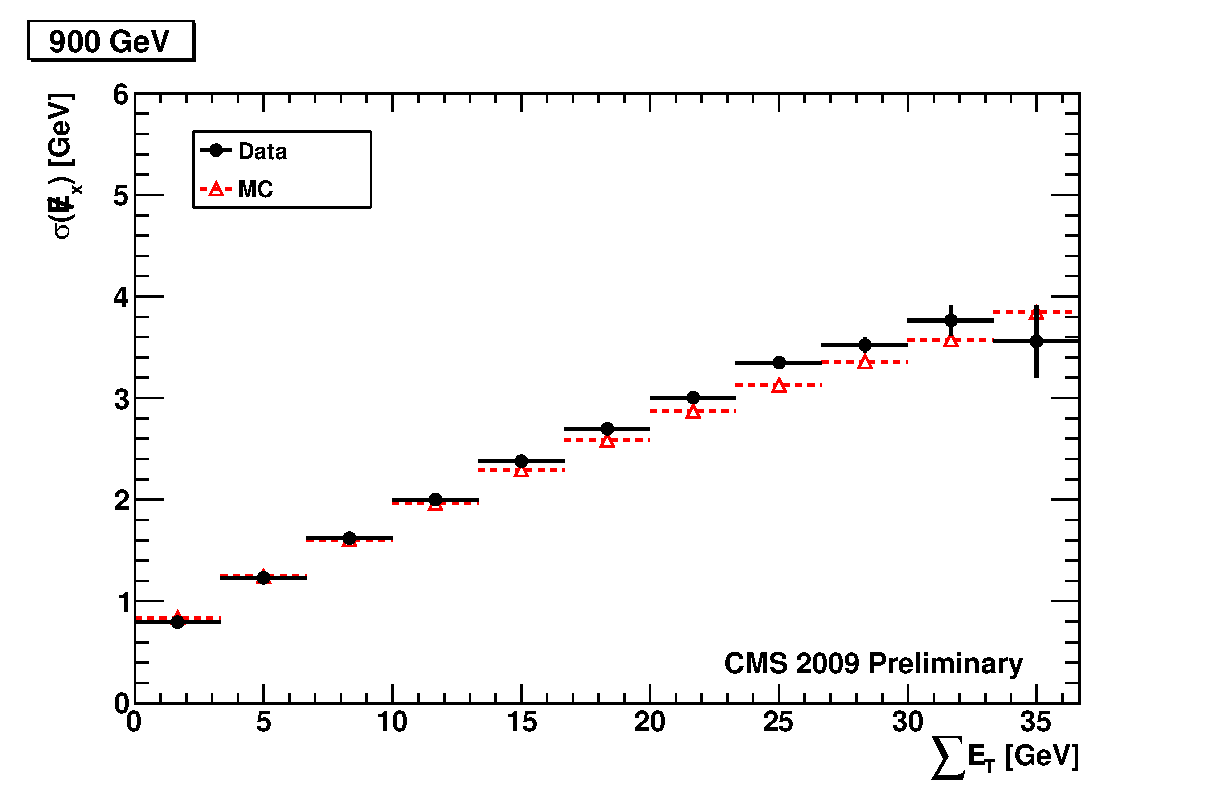
\includegraphics[width=0.5\textwidth]{plots_DataVsMC_MB_900GeV/h_metxsigma_sumet_900.eps} &
  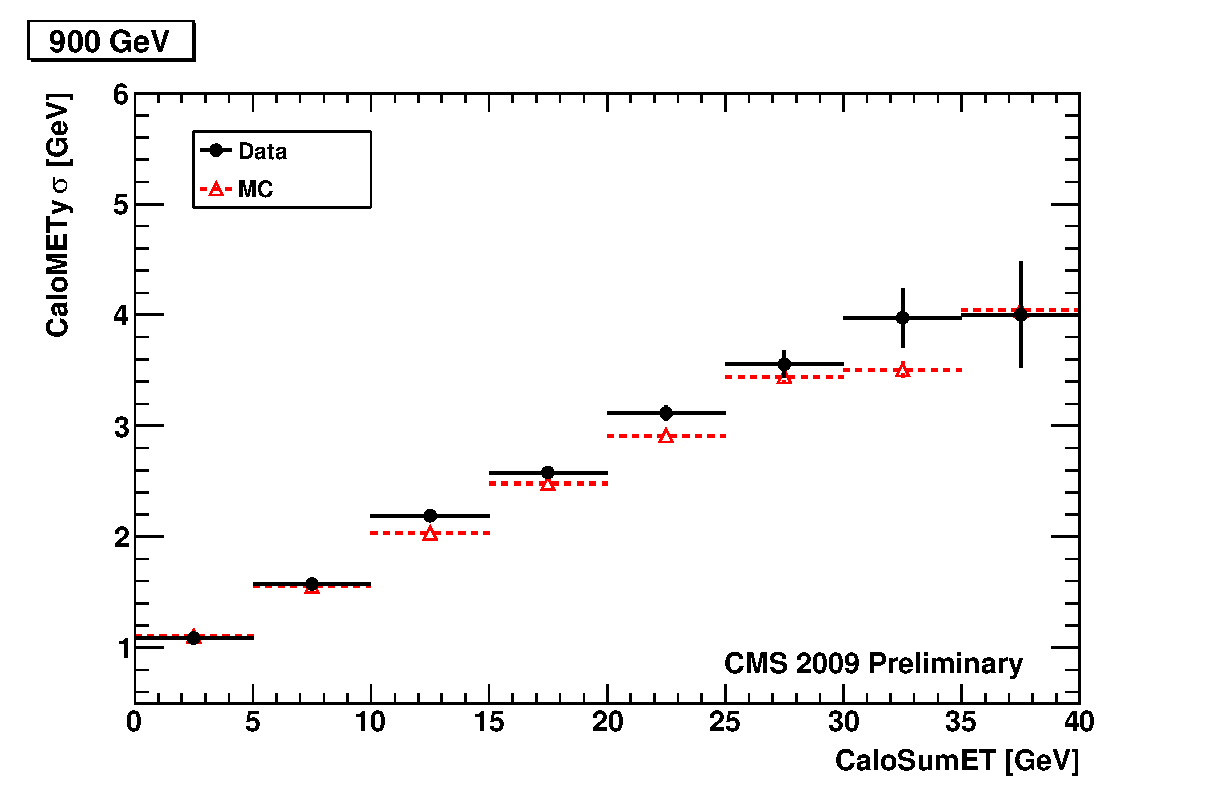
\includegraphics[width=0.5\textwidth]{plots_DataVsMC_MB_900GeV/h_metysigma_sumet_900.eps} \\
 \end{tabular}
 \caption{\small Comparison of the $\exmiss$ $\sigma$ vs. $\sum E_\text{T}$ and $\eymiss$ $\sigma$ vs. $\sum E_\text{T}$ between 
          Monte Carlo and data at $900$ GeV.\label{fig:MExySigma_vs_SumET_900}}
\end{figure}

\begin{figure}[h!]
 \centering
 \begin{tabular}{ll}
  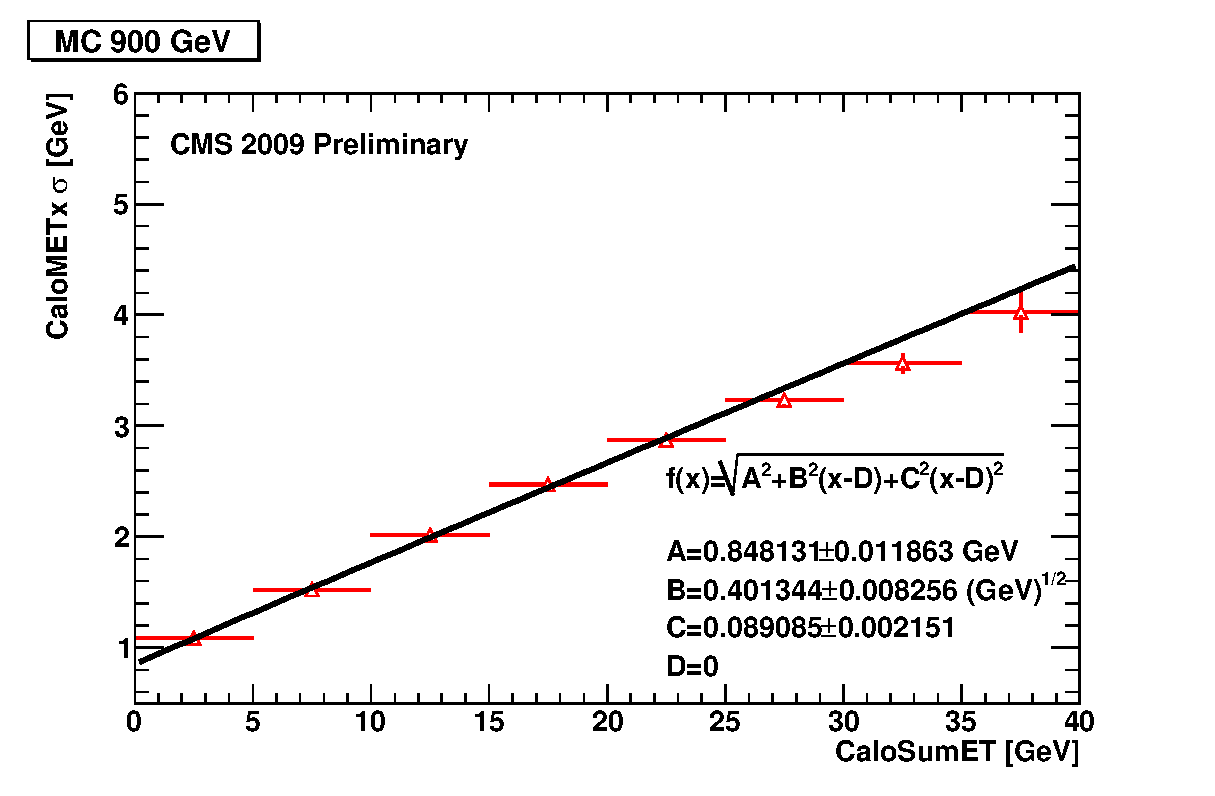
\includegraphics[width=0.5\textwidth]{plots_DataVsMC_MB_900GeV/final_metxsigma_sumet_MC_900.eps} &
  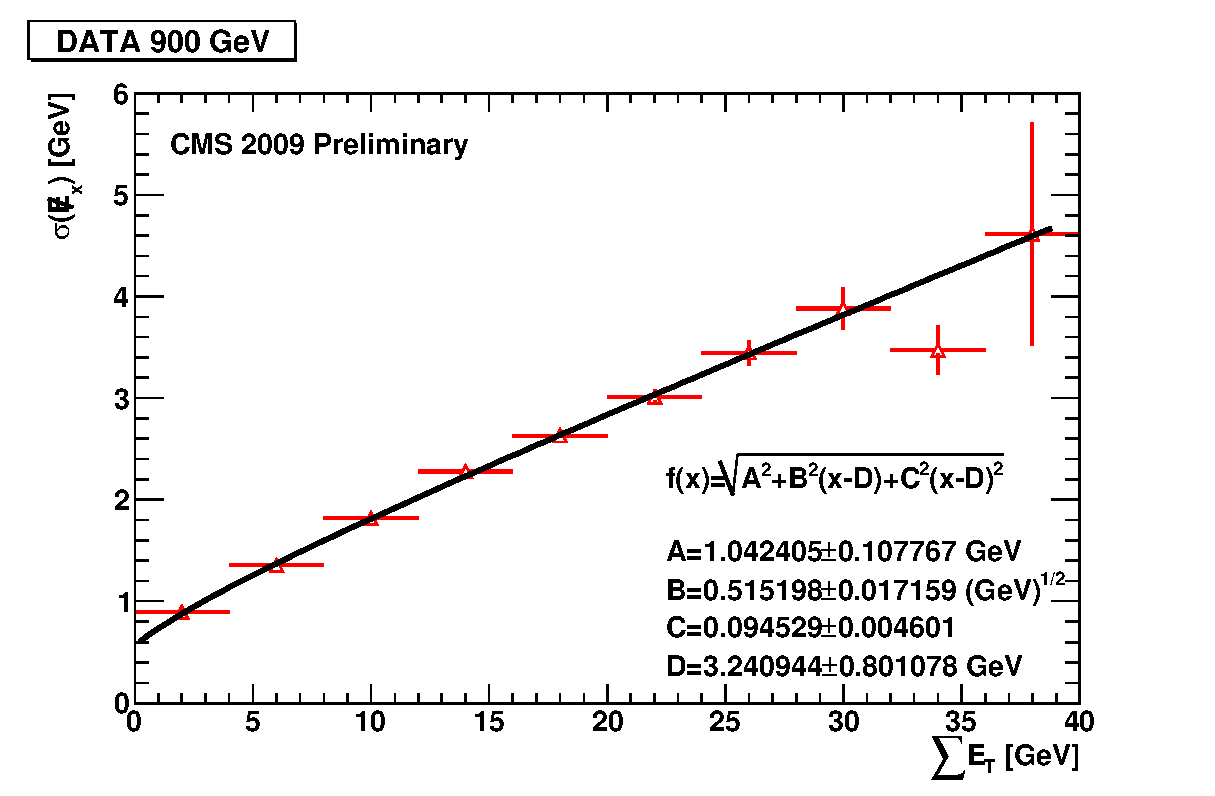
\includegraphics[width=0.5\textwidth]{plots_DataVsMC_MB_900GeV/final_metxsigma_sumet_DATA_900.eps} \\
 \end{tabular}
 \caption{\small Fit of the $\exmiss$ $\sigma$ vs. $\sum E_\text{T}$ for Monte Carlo and data at $900$ GeV. Parameter $D$ in the fit was fixed
          to zero.\label{fig:MExSigma_vs_SumET_900_fit}}
\end{figure}

\begin{figure}[h!]
 \centering
 \begin{tabular}{ll}
  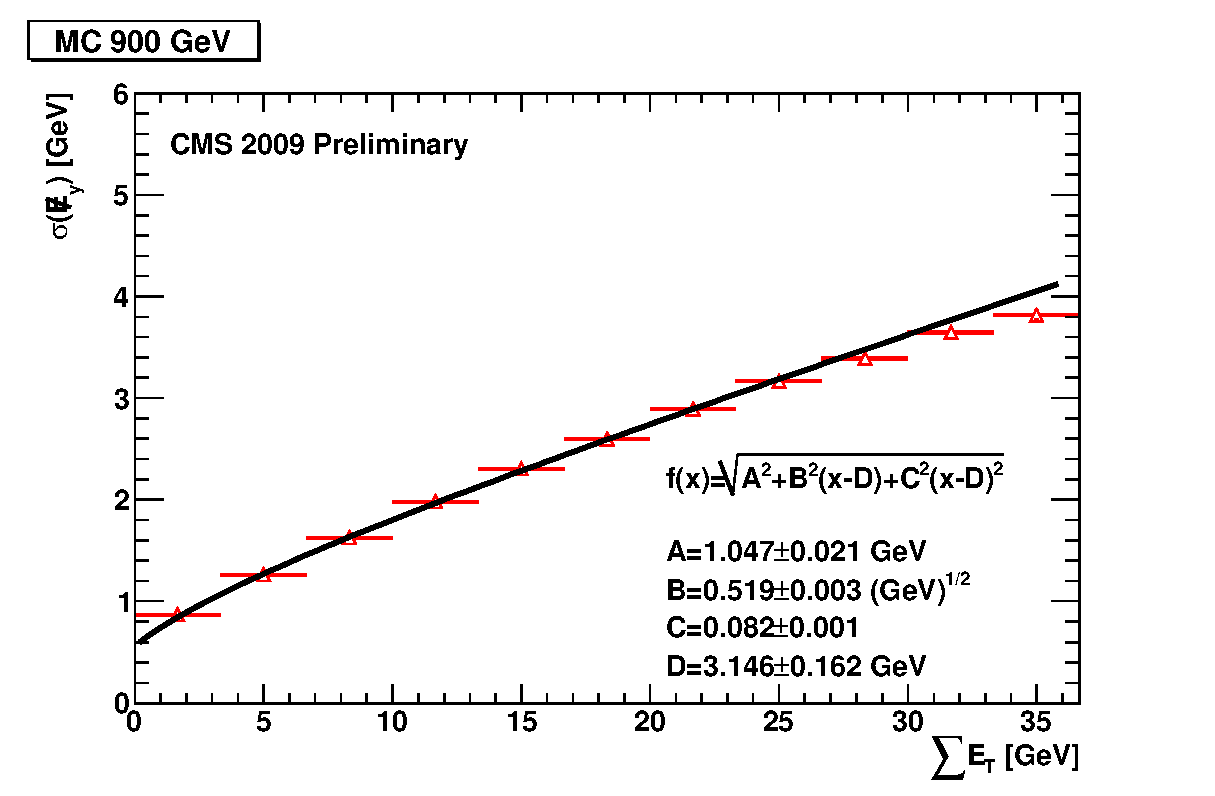
\includegraphics[width=0.5\textwidth]{plots_DataVsMC_MB_900GeV/final_metysigma_sumet_MC_900.eps} &
  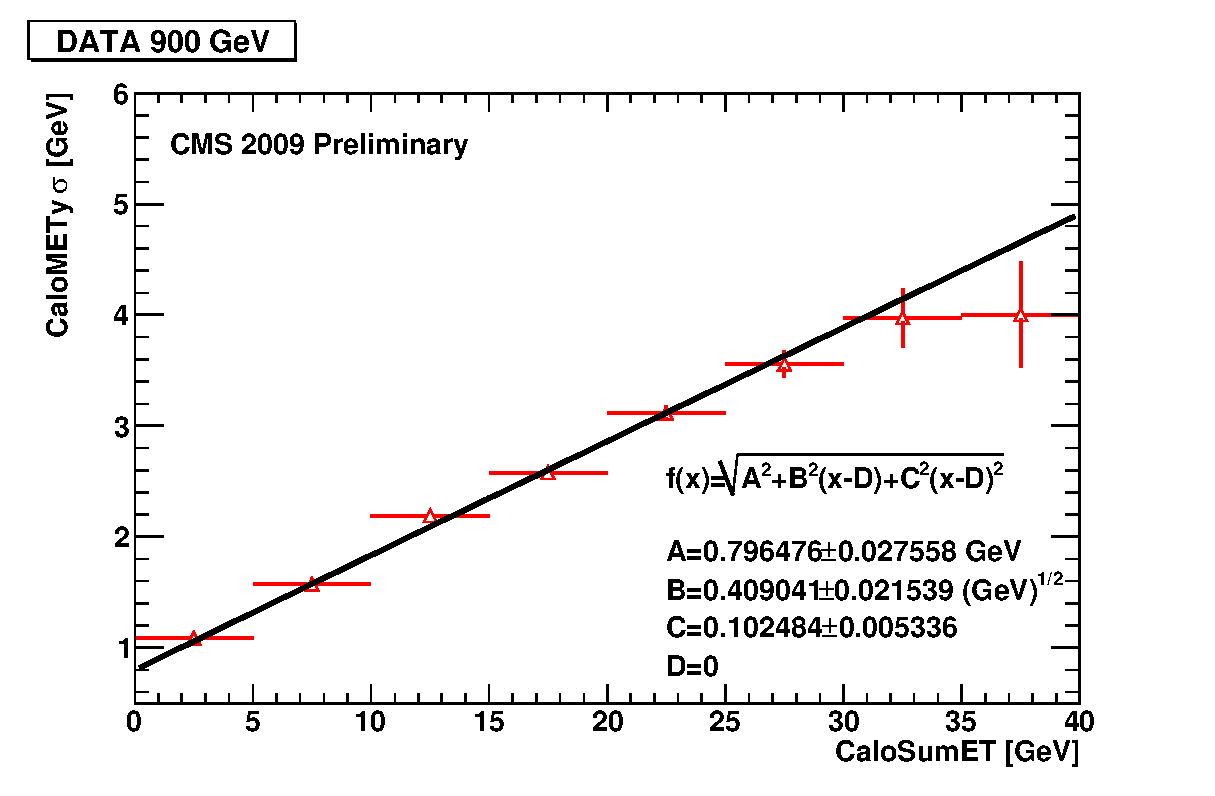
\includegraphics[width=0.5\textwidth]{plots_DataVsMC_MB_900GeV/final_metysigma_sumet_DATA_900.eps} \\
 \end{tabular}
 \caption{\small Fit of the $\eymiss$ $\sigma$ vs. $\sum E_\text{T}$ for Monte Carlo and data at $900$ GeV. Parameter $D$ in the fit was fixed
          to zero.\label{fig:MExSigma_vs_SumET_900_fit}}
\end{figure}

\clearpage

\subsection{$\etmiss$ and SumET dependence on $\eta$}

\begin{figure}[h!]
 \centering
 \begin{tabular}{ll}
  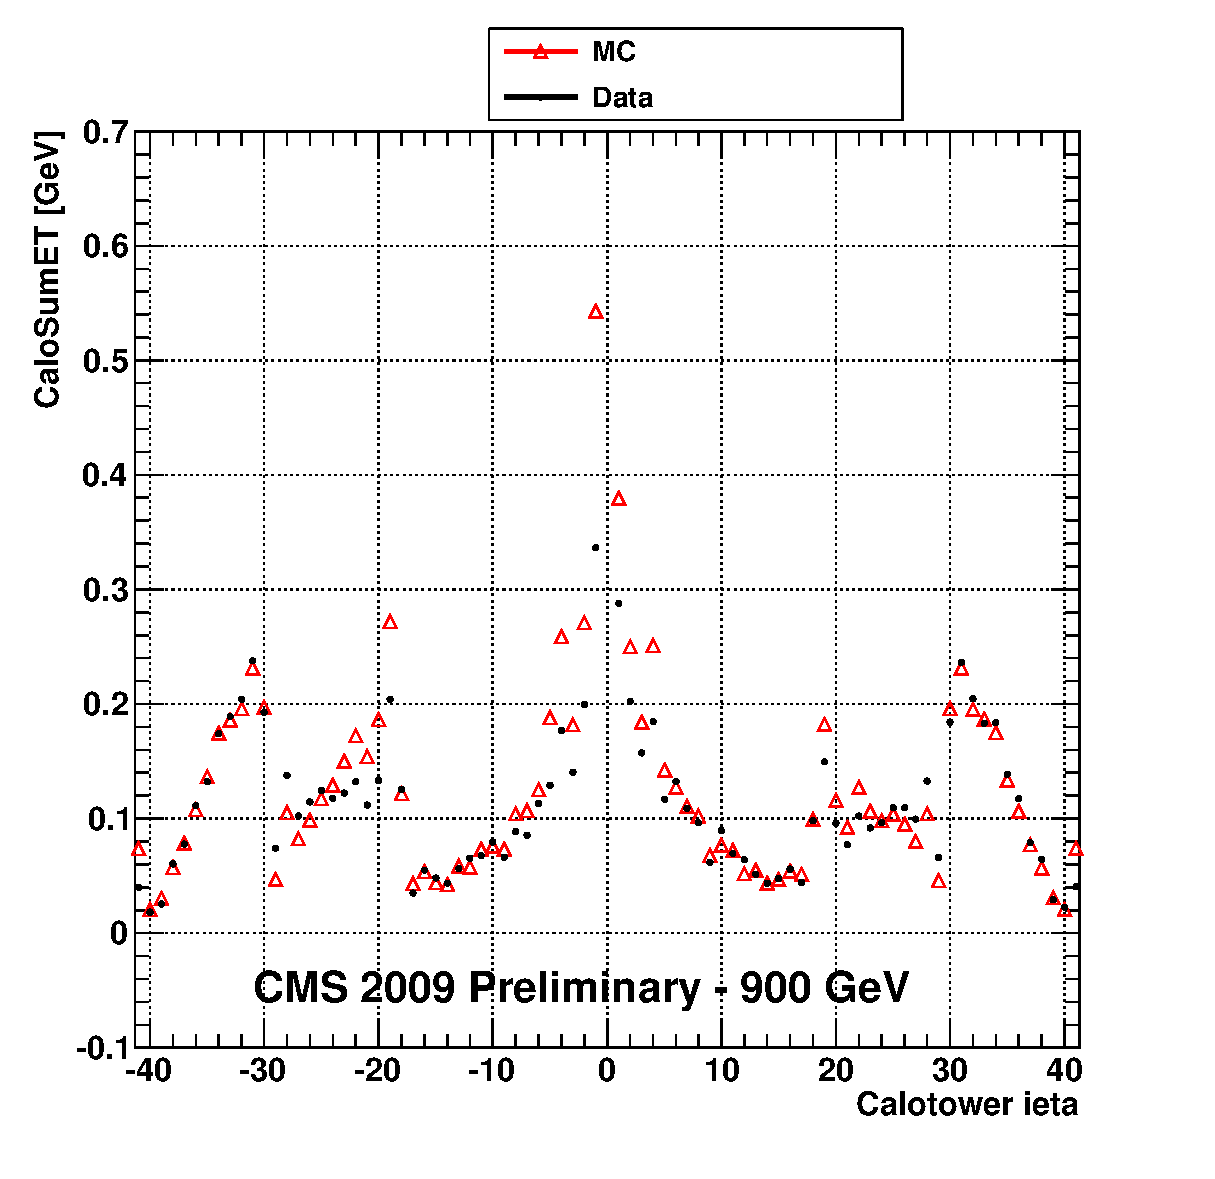
\includegraphics[width=0.5\textwidth]{plots_DataVsMC_MB_900GeV/g_caloSumetMean_vs_ieta_900.eps} &
  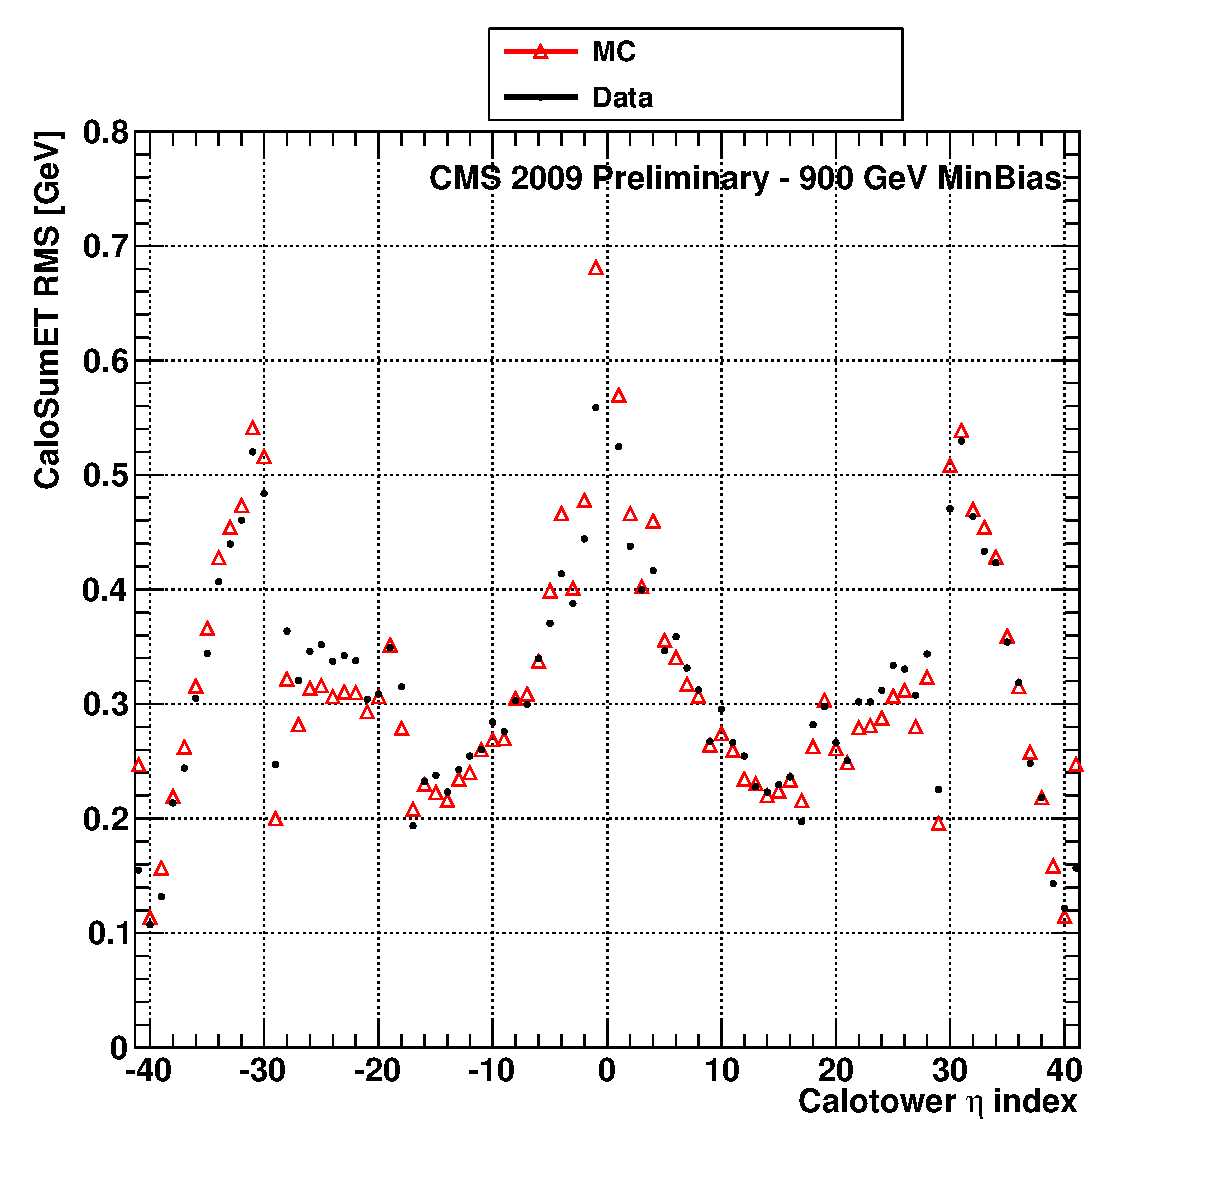
\includegraphics[width=0.5\textwidth]{plots_DataVsMC_MB_900GeV/g_caloSumetRMS_vs_ieta_900.eps} \\
 \end{tabular}
 \caption{\small Comparison of the SumET Mean vs. i$\eta$ of calotowers and SumET RMS vs. i$\eta$ of calotowers between 
          Monte Carlo and data at $900$ GeV.\label{fig:SumET_MeanRMS_vs_ieta_900}}
\end{figure}

\begin{figure}[h!]
 \centering
 \begin{tabular}{ll}
  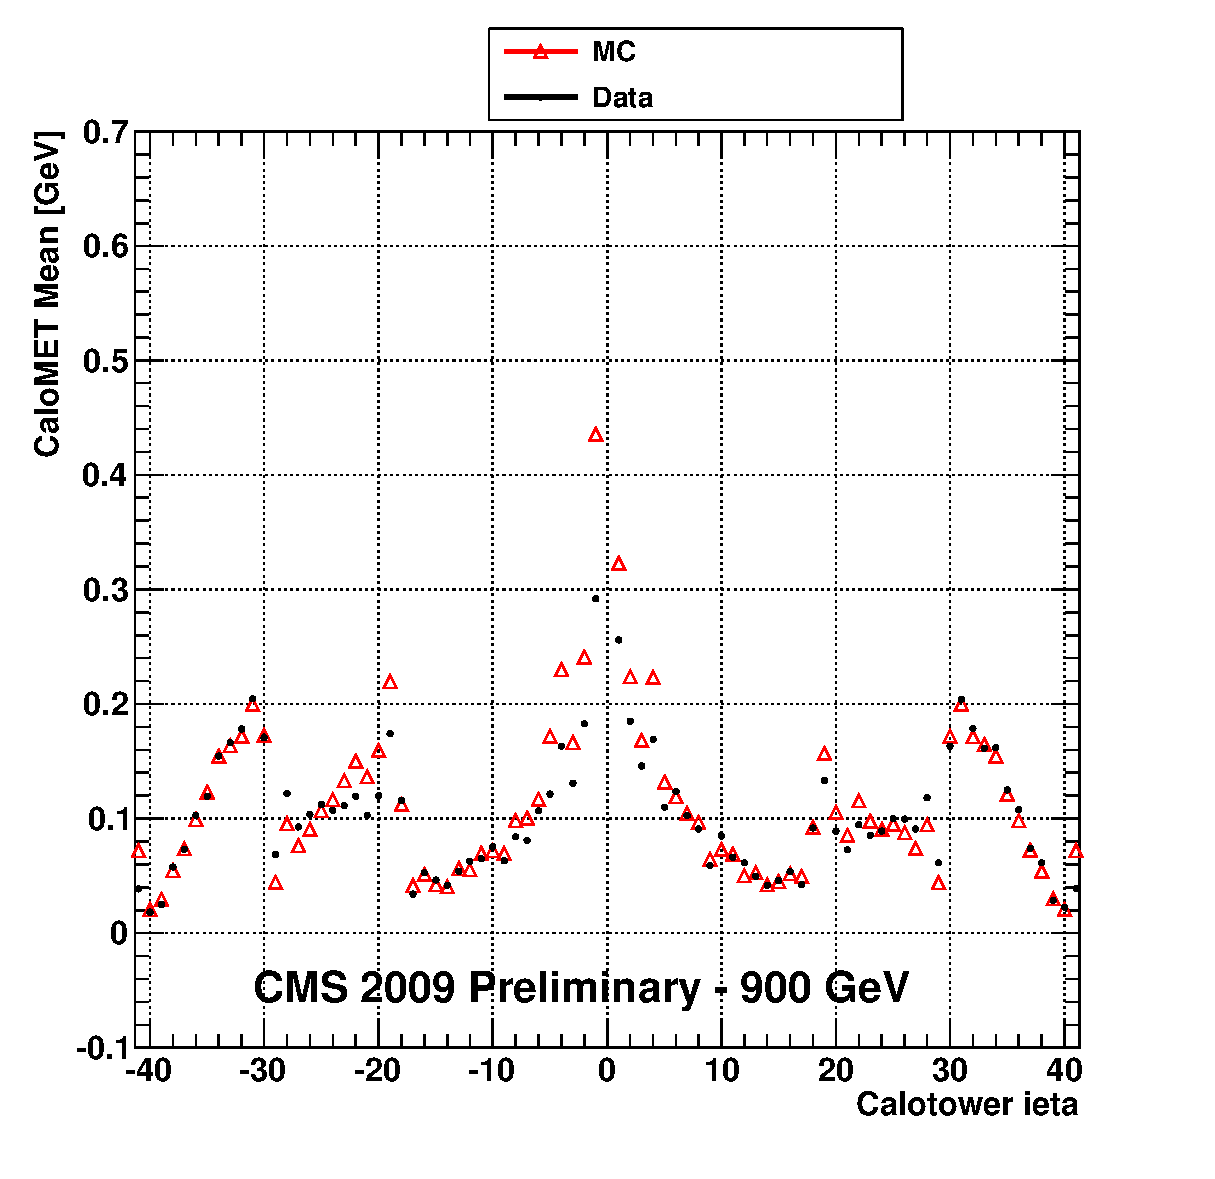
\includegraphics[width=0.5\textwidth]{plots_DataVsMC_MB_900GeV/g_calometPtMean_vs_ieta_900.eps} &
  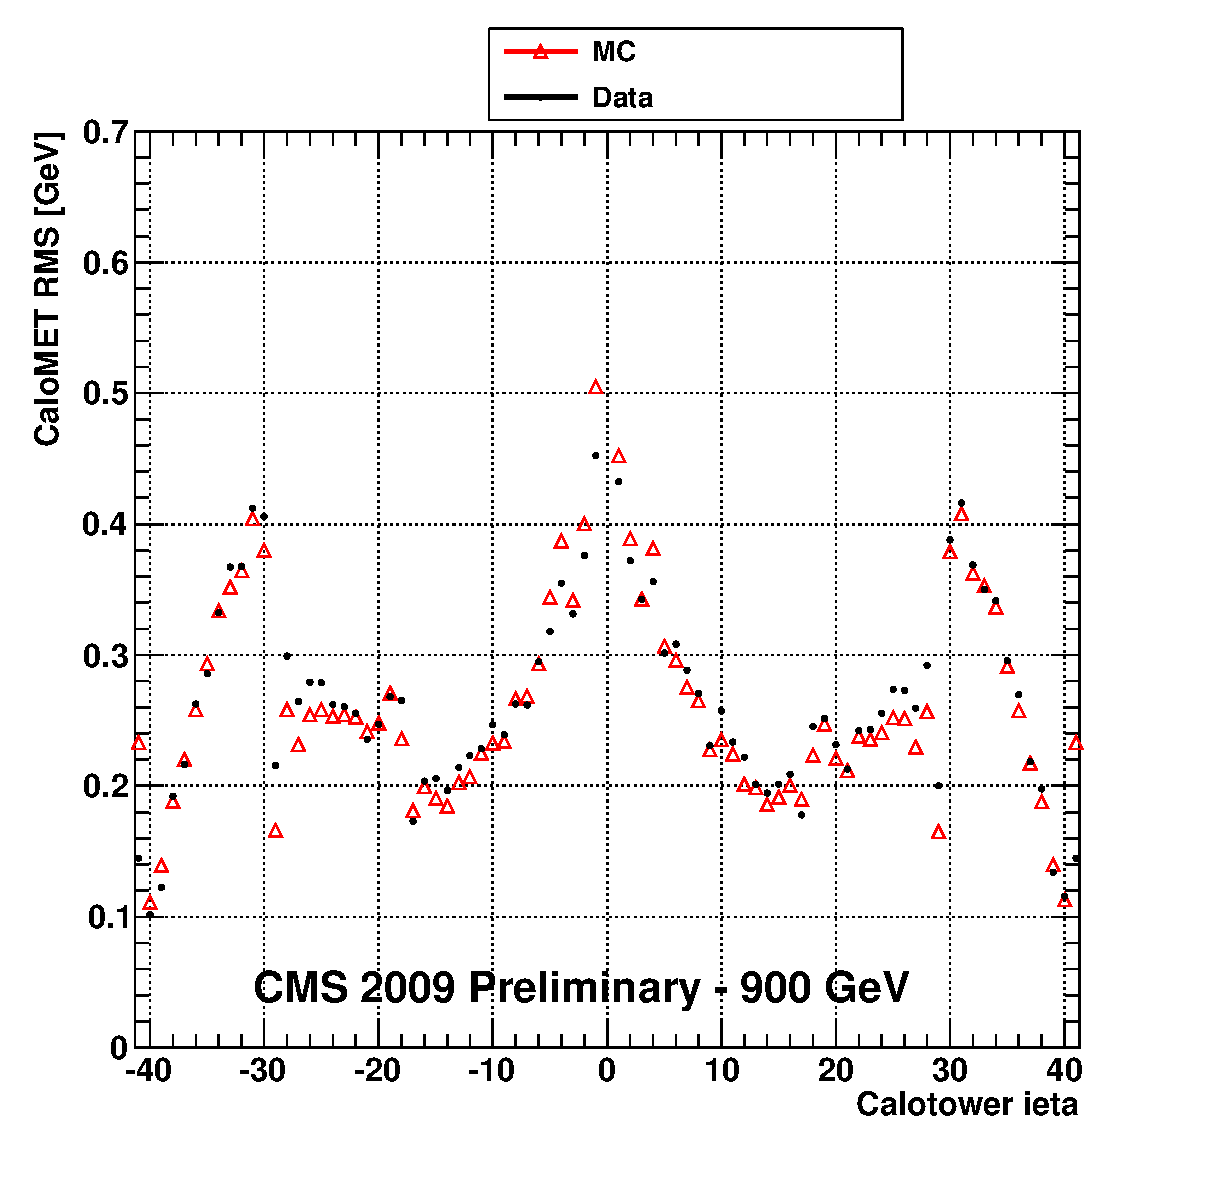
\includegraphics[width=0.5\textwidth]{plots_DataVsMC_MB_900GeV/g_calometPtRMS_vs_ieta_900.eps} \\
 \end{tabular}
 \caption{\small Comparison of the $\etmiss$ Mean vs. i$\eta$ of calotowers and $\etmiss$ RMS vs. i$\eta$ of calotowers between 
          Monte Carlo and data at $900$ GeV.\label{fig:MET_MeanRMS_vs_ieta_900}}
\end{figure}

\begin{figure}[h!]
 \centering
 \begin{tabular}{ll}
  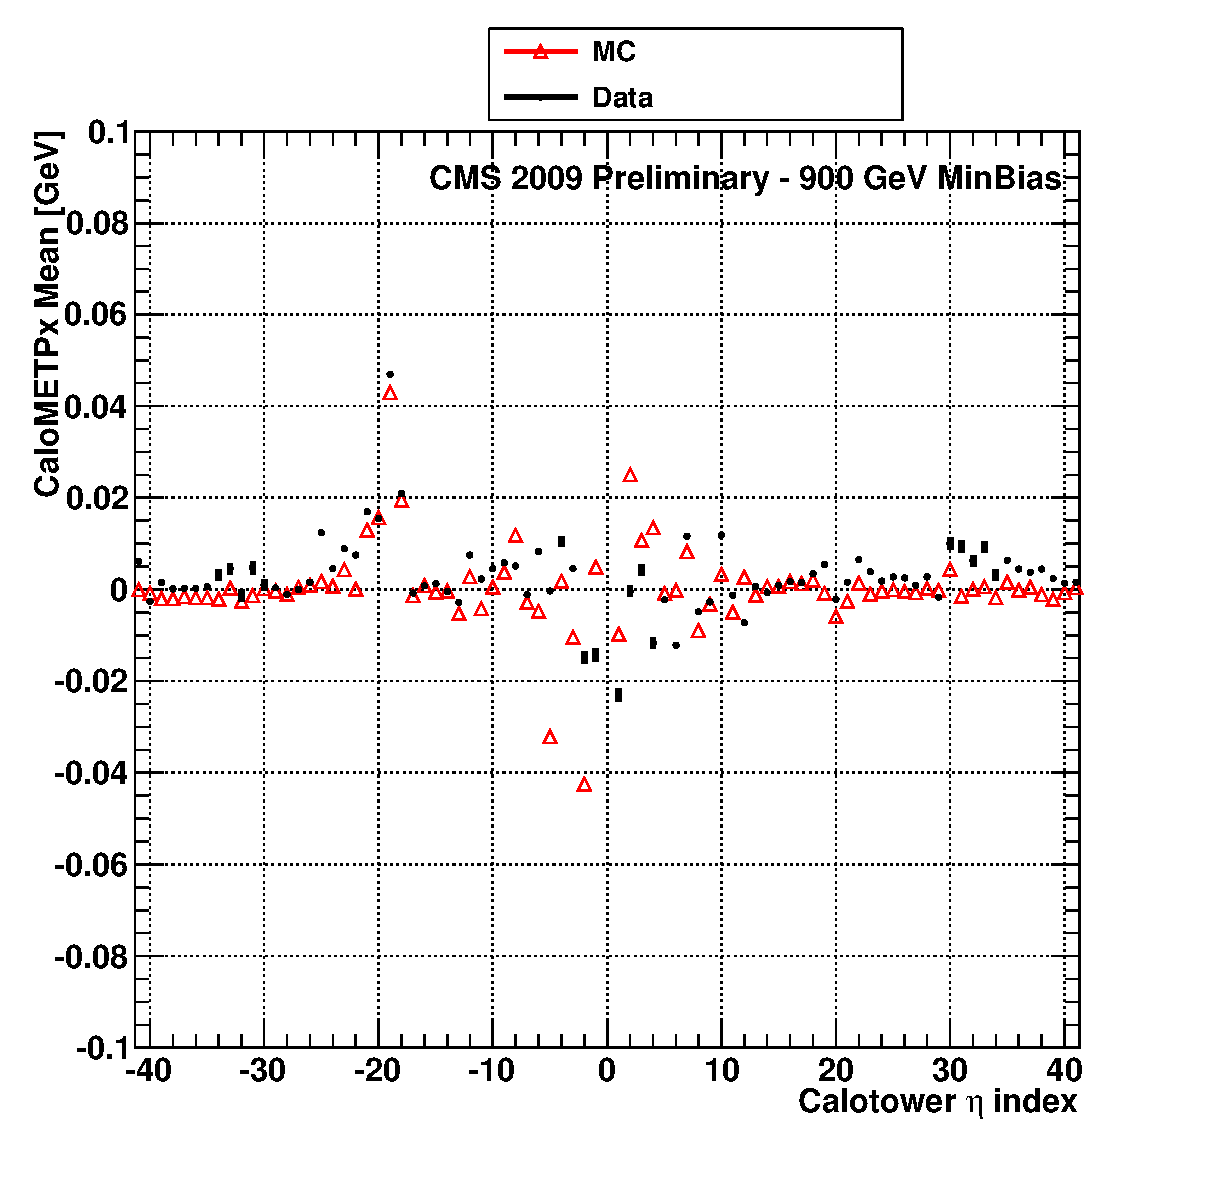
\includegraphics[width=0.5\textwidth]{plots_DataVsMC_MB_900GeV/g_calometPxMean_vs_ieta_900.eps} &
  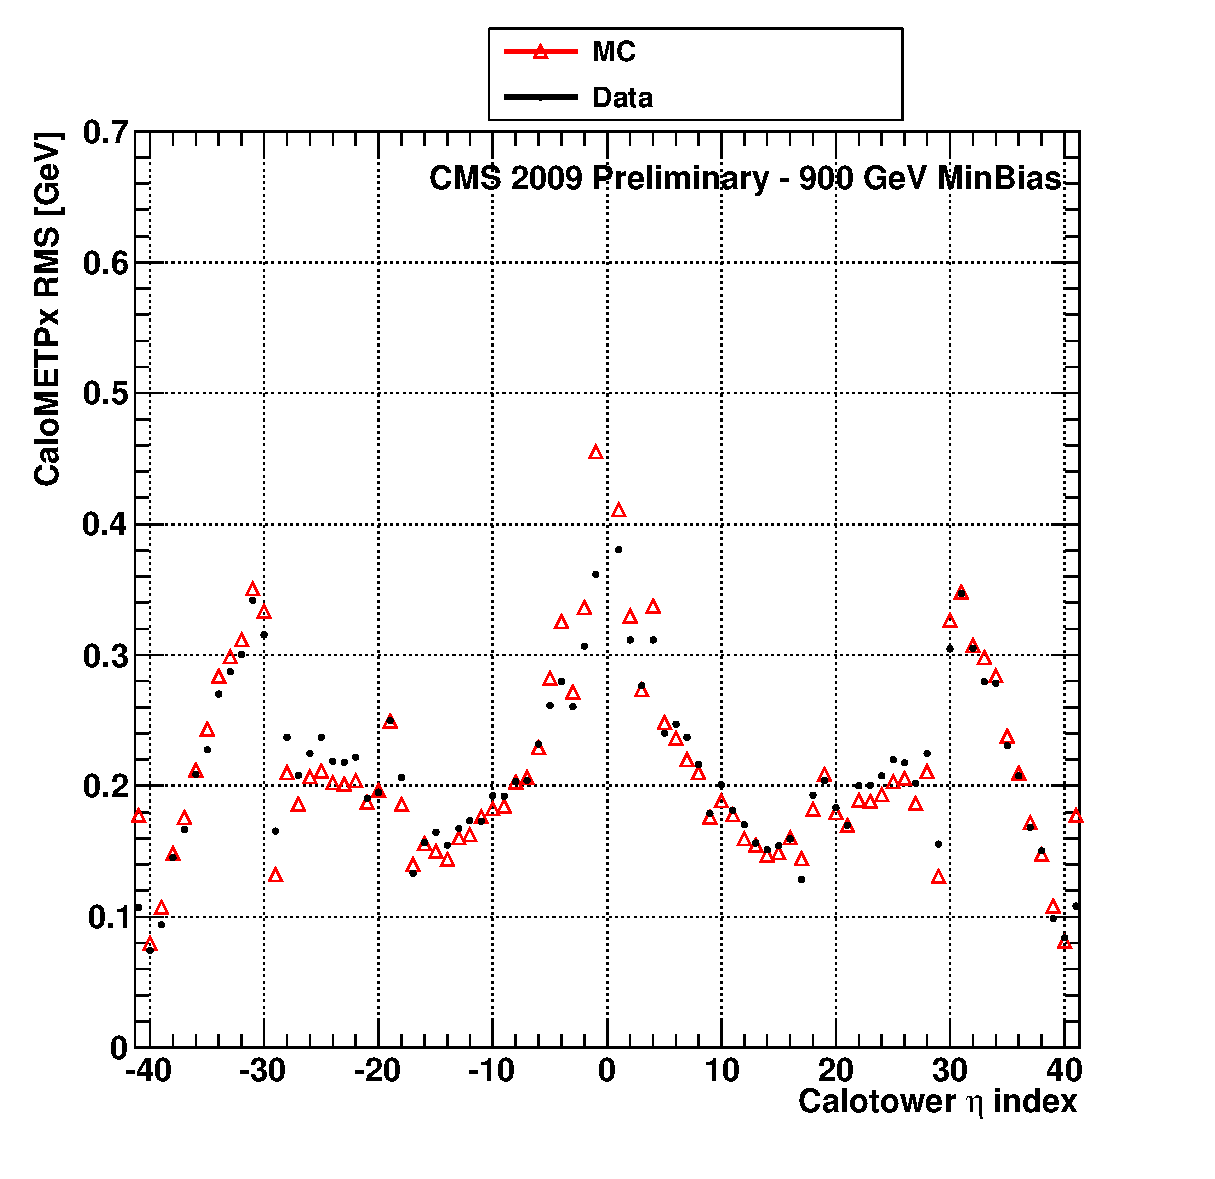
\includegraphics[width=0.5\textwidth]{plots_DataVsMC_MB_900GeV/g_calometPxRMS_vs_ieta_900.eps} \\
 \end{tabular}
 \caption{\small Comparison of the $\exmiss$ Mean vs. i$\eta$ of calotowers and $\exmiss$ RMS vs. i$\eta$ of calotowers between 
          Monte Carlo and data at $900$ GeV.\label{fig:METx_MeanRMS_vs_ieta_900}}
\end{figure}

\begin{figure}[h!]
 \centering
 \begin{tabular}{ll}
  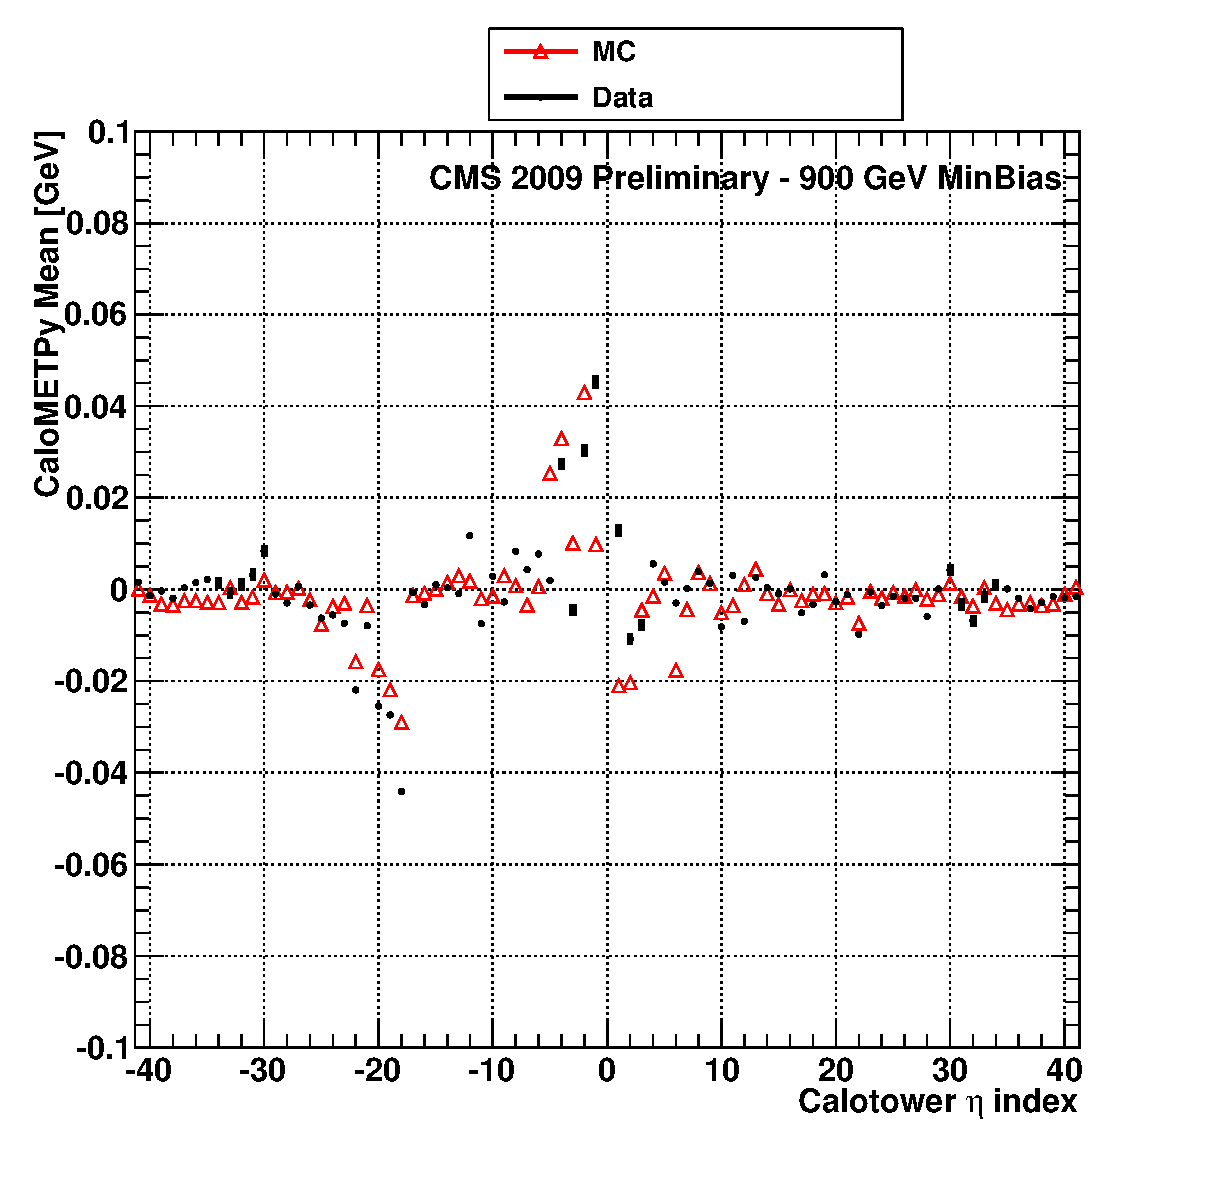
\includegraphics[width=0.5\textwidth]{plots_DataVsMC_MB_900GeV/g_calometPyMean_vs_ieta_900.eps} &
  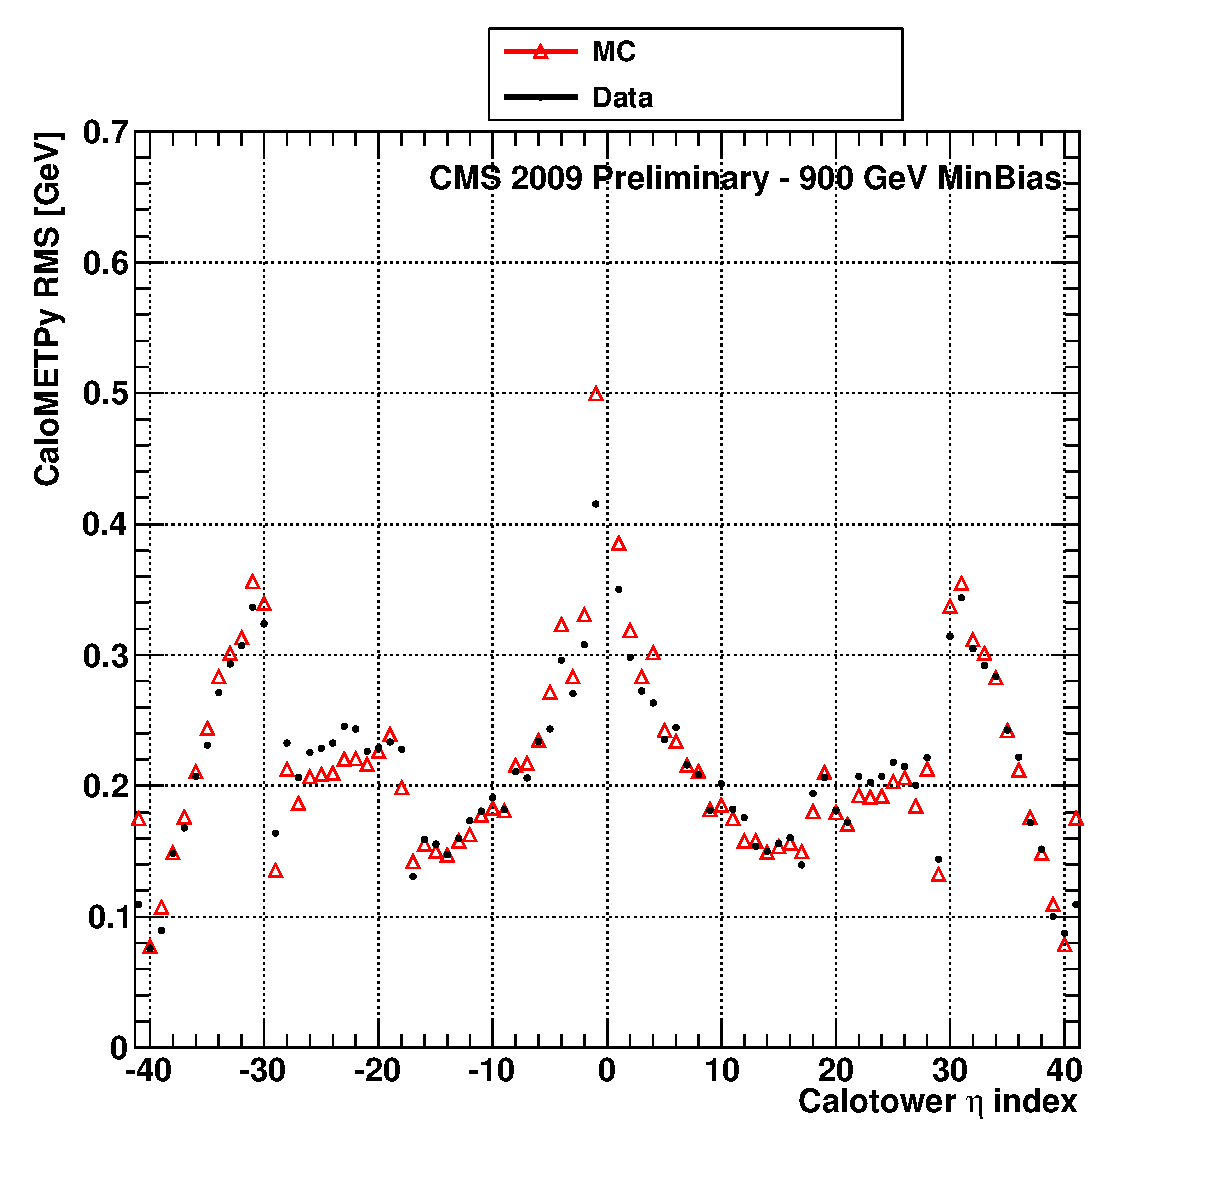
\includegraphics[width=0.5\textwidth]{plots_DataVsMC_MB_900GeV/g_calometPyRMS_vs_ieta_900.eps} \\
 \end{tabular}
 \caption{\small Comparison of the $\eymiss$ Mean vs. i$\eta$ of calotowers and $\eymiss$ RMS vs. i$\eta$ of calotowers between 
          Monte Carlo and data at $900$ GeV.\label{fig:METy_MeanRMS_vs_ieta_900}}
\end{figure}

\clearpage
